
Une agence de voyage propose deux formules week-end pour se rendre à Londres au départ de Nantes. Les clients choisissent leur moyen de transport : train ou avion. De plus, s’ils le souhaitent, ils peuvent compléter leur formule par l’option « visites guidées ». Une étude a produit les données suivantes :

\begin{itemize}
	\item 40 \% des clients optent pour l’avion;
	\item parmi les clients ayant choisi le train, 50 \% choisissent aussi l’option « visites guidées »;
	\item 12 \% des clients ont choisi à la fois l’avion et l’option « visites guidées ».
\end{itemize}

On interroge au hasard un client de l’agence ayant souscrit à une formule week-end à Londres. On considère les évènements suivants :

\begin{itemize}
	\item $A$ : « le client a choisi l’avion »;
	\item $V$ : « le client a choisi l’option « visites guidées » ».
\end{itemize}

\begin{enumerate}
	\item 	De l’énoncé on déduit que :
	
	\[
	\begin{array}{l}
		P(A) = 0,4; \\
		P_{\overline{A}}(V) = 0,5; \\
		P(A \cap V) = 0,12.
	\end{array}
	\]
	
	On a donc $P_{\overline{A}}(V) = \dfrac{P(A \cap V)}{P(A)} = \dfrac{0,12}{0,4} = \dfrac{12}{40} = \dfrac{3}{10} = 0,3$.
	
	\item
	On peut dresser un arbre pondéré de probabilités :\\
	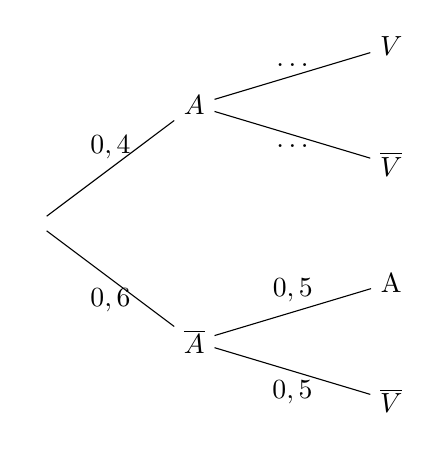
\begin{tikzpicture}
		[level 1/.style={level distance=2cm,
			sibling distance=3cm},
		level 2/.style={level distance=2.5cm,
			sibling distance=1.5cm}]
		\node {} [grow'=right]
		child {node {$A$}
			child {node {$V$}
				edge from parent node[above] {$\ldots$}
			}
			child {node {$\overline V$}
				edge from parent node[below] {$\ldots$}
			}
			edge from parent node[above] {$0,4$}
		}
		child {node {$\overline A$}
			child {node {A}
				edge from parent node[above] {$0,5$}
			}
	child {node {$\overline V$}
		edge from parent node[below] {$0,5$}
	}
	edge from parent node[below] {$0,6$}
	}
	;
	\end{tikzpicture}
	
	D’après la loi des probabilités totales :
	\[
	P(V) = P(A \cap V) + P(\overline{A} \cap V).
	\]
	
	Or $P(\overline{A} \cap V) = P(\overline{A}) \times P_{\overline{A}}(V) = 0,6 \times 0,5 = 0,3$ 
	
	Donc $P(V) = 0,12 + 0,30 = 0,42$.
	
	\item
	Calculer la probabilité pour que le client interrogé ait pris l’avion sachant qu’il n’a pas choisi l’option « visites guidées ». Arrondir le résultat au centième.
	
	On a $P_{\overline{V}}(A) = \dfrac{P(\overline{V} \cap A)}{P(\overline{V})} = \dfrac{P(A \cap \overline{V})}{P(\overline{V})}$.
	
	Or d’après la question précédente : \\
	$P(\overline{V}) = 1 - P(V) = 1 - 0,42 = 0,58$\\
	 et d’après la question 1 :\\
	  $P_{\overline{A}}(V) = 1 - P_{\overline{A}}(V) = 1 - 0,3 = 0,7$.
	
	Donc $P_{\overline{V}}(A) = \dfrac{0,4 \times 0,7}{0,58} = \dfrac{0,28}{0,58} = \dfrac{28}{58} = \dfrac{14}{29} \approx 0,482$, soit $0,48$ au centième près.
	
	\item
	On interroge au hasard deux clients de manière aléatoire et indépendante. Quelle est la probabilité qu’aucun des deux ne prenne l’option « visites guidées » ?
	
	On a vu que $P(\overline{V}) = 1 - 0,42 = 0,58$. La probabilité cherchée est donc égale à $0,58 \times 0,58 = 0,3364$.
\end{enumerate}


